\documentclass[times, utf8, numeric]{fer}
\usepackage{booktabs}
\usepackage{url}
\usepackage{float}
\usepackage{pdfpages}
\usepackage{hyperref}

\begin{document}

\begin{titlepage}
	\centering
	{\scshape\LARGE Fakultet elektrotehnike i računarstva \par}
	\vspace{1cm}
	{\scshape\Large Preddiplomski projekt\par}
	\vspace{1.5cm}
	{\huge\bfseries Robot Robby\par}
	\vspace{2cm}
	{\Large\itshape
	Dominik Stanojević \par
	Leon Luttenberger \par
	Domagoj Pluščec \par
	Dunja Vesinger \par
	Kristijan Vulinović\par}
	\vfill
	Mentor:\par
	Doc. dr. sc. Marko \textsc{Čupić}
	\vfill	
	Verzija: 1.0
	\vfill

% Bottom of the page
	{\large \today\par}
\end{titlepage}

\pagebreak
\tableofcontents

\pagebreak
\pagenumbering{arabic}

\chapter{Informacije o projektu}
\section{Puni naziv projekta}

\section{Skraćeni naziv projekta}

\section{Opis projekta}
Ovaj projekt bavi se izradom "mozga" jednostavnog robota. Ideja robota, originalno nazvanog Robby, preuzeta je iz knjige Complexity: A Guided Tour autorice Melanie Mitchell. Robby živi u dvodimenzionalnom svijetu unutar kojeg su razbacane limenke i njegova je osnovna zadaća sakupiti ih ove limenke kako bi očistio svoj svijet. No, Robby ima ograničenu bateriju što znači da mu je na raspolaganju ograničen unutar jedne sesije čišćenja. Stoga je potrebno pažljivo odabrati koje će akcije robot izvoditi kako bi sakupio što više limenki prije nego što ostane bez baterije.
\vspace{1ex}\\ 
Svijet u kojem Robby živi pravokutnog je oblika i okružen je zidovima kroz koje robot ne može proći. Podijeljen je u ćelije po kojima se Robby može kretati. Na svakoj od ćelija može se nalaziti najviše jedna limenka. Unutar svih rubnih ćelija nalaze se zidovi i na njima ne mogu biti limenke. Robot se na početku svake sesije nalazi u jednoj nasumce odabranoj ćeliji. Ima unaprijed određen broj poteza koje može izvesti u jedno sesiji čišćenja i u svakom potezu može poduzeti jednu od sedam ponuđenih akcija: pomakni se jedu ćeliju sjeverno, južno, istočno ili zapadno, pokupi limenku s trenutne ćelije, nemoj učiniti ništa ili poduzmi nasumičnu akciju.  
\vspace{1ex}\\
No, Robby nema mogućnost pamćenja. Može donjeti odluku o tome koju će akciju poduzeti samo na temelju trenutne percepcije. U svakom trenutku robot vidi sadržaj ukupno pet ćelija: ćelije na kojoj stoji te ćelija koje su sjeverno, južno, istočno i zapadno od njega. Cilj ovog projekta je uporabom različitih algoritama pronaći što bolju strategiju odabira robotovog sljedećeg poteza na temelju sadržaja ovih pet ćelija.
\vspace{1ex}\\
Mozak robota razvija se sljedećim pristupima:
\begin{itemize}
	\item izravnim kodiranjem percepcija-akcija koje se uči genetskim algoritmom;
	\item unaprijednom umjetnom neuronskom mrežom koja se uči evolucijskim algoritmom;
	\item Elmannovom umjetnom neuronskom mrežom koja se uči evolucijskim algoritmom;
	\item genetskim programiranjem;
	\item podržanim učenjem.
\end{itemize}
\vspace{1ex}
Navedeni pristupi trebaju način procjene kvalitete strategije robota, stoga je potrebno izgraditi simulator. U okviru projekta izađuju se dva simulatora: negrafički i grafički. Negrafički simulator služi za simulaciju ponašanja robota s ciljem dobovanja statističkih podataka o sesijama čišćenja za potrebe algoritama koji razvijaju strategije robota. Grafički simulator ima grafičko sučelje koje omogućava animirani prikaz rada robota koji slijedi odabranu strategiju na mapi.
\vspace{1ex}\\
U okviru projekta realizira se i grafičko sučelje kroz koje je moguće trenirati mozak robota odabranim pristupom. Za svaki je pristup moguće podesiti njemu odgovarajuće parametre te pratiti napredak učenja robota kroz izvođenje algoritma. Strategiju kojom treniranje rezultira moguće je pohraniti u datoteku. Također je moguće učitati prethodno pohranjenu strategiju i prikazati njezino ponašanje na raznim mapama u simulatoru.
\\
Svi segmenti projekta izrađuju se u programskom jeziku Java.

\section{Cilj projekta}

\section{Voditelj studentskog tima}
Voditelj: Dominik Stanojević

\section{Rezultati}
\section{Slični projekti}

\chapter{Organizacija projekta}
\section{Resursi}
U sklopu ovog projekta bit će korišteni sljedeći resursi:
\begin{enumerate}
	\item \begin{flushleft}\textbf{Ljudski resursi.}\end{flushleft}
	Projekt će izvoditi tim od pet studenata FER-a čije su informacije navedene u tablici ljudskih resursa (tablica 			\ref{table:ljudstvo}).
	
	\begin{table}[H]
	\centering
 	\begin{tabular}{|l l l|} 
 	\hline
 	Ime i prezime & E-mail adresa & Napomena\\ [0.5ex] 
	\hline
 	Leon Luttenberger & \href{mailto:leon.luttenberger@fer.hr}{leon.luttenberger@fer.hr} & \\
 	Domagoj Pluščec & \href{mailto:domagoj.pluscec@fer.hr}{domagoj.pluscec@fer.hr} & \\
 	Dominik Stanojević & \href{mailto:dominik.stanojevic@fer.hr}{dominik.stanojevic@fer.hr} & 
 	voditelj projektnog tima\\
 	Dunja Vesinger & \href{mailto:dunja.vesinger@fer.hr}{dunja.vesinger@fer.hr} & \\
 	Kristijan Vulinović & \href{mailto:kristijan.vulinovic@fer.hr}{kristijan.vulinovic@fer.hr} & \\
 	\hline
 	\end{tabular}
 	\caption{Ljudski resursi}
	\label{table:ljudstvo}
	\end{table}
	
	\item \begin{flushleft}\textbf{ Materijalni resursi:} \end{flushleft}
	\begin{enumerate}
		\item \begin{flushleft}\textbf{Računalni resursi}\end{flushleft}
		Studenti uključeni u projekt koristit će svoja i fakultetska računala kako bi ostvarili projekt.
		
		\item \begin{flushleft}\textbf{Programski alati}\end{flushleft}
		U sklopu projekta koristit će se sustav za upravljanje izvornim kodom Git te Internet spremište 				Github. Za potrebe pisanja programskog koda sudionici će koristiti razvojne okoline Eclipse i IntelliJ IDEA. Za komunikaciju unutar tima koristit ćemo web alat za timsku komunikaciju Slack te za potrebe 	praćenja napretka projekta koristit ćemo alat za praćenje napretka Trello.
\end{enumerate}
\end{enumerate}

\section{Glavni rizici}
U tablici rizika (tablica \ref{table:glavni}) navedeni su rizici i njihove važnosti za izvedbu projekta.

\begin{table}[H]
	\centering
 	\begin{tabular}{|l l l|} 
 	\hline
 	Identifikator rizika & Rizik & Razina rizika\\ [0.5ex] 
	\hline
 	R1 & \begin{tabular}{@{}l@{}}Nedostupnost jednog ili više članova  \\ 
 		tima u nekoj fazi projekta.\end{tabular} & visoka\\
 	R2 & Odstupanje od zadanih rokova. & visoka\\
 	R3 & \begin{tabular}{@{}l@{}}Tehničke pogreške \\ 
 		(npr. slučajno brisanje lokalno spremljenih podataka)\end{tabular}& srednja\\
 	R4 & Nedostatak komunikacije među članovima & srednja\\
 	R5 & Pogrešno razumijevanje zadanog zadatka& srednja\\
 	R6 & Pogrešna implementacija podzadatka & srednja\\
 	R7 & \begin{tabular}{@{}l@{}}Rizici pri službenoj predaji dokumenta  \\ 
 		(npr. nedostupnost web sjedišta fer.hr)\end{tabular}& niska\\
 	R8 & Nedostatak znanja za izradu određenog zadatka & niska\\
 	\hline
 	\end{tabular}
 	\caption{Glavni rizici}
	\label{table:glavni}
	\end{table}

\section{Smanjivanje rizika}
Tablica dana u nastavku prikazuje postupke za smanjivanje rizika (tablica \ref{table:smanjivanje}).
\begin{table}[H]
	\centering
 	\begin{tabular}{|l l|} 
 	\hline
 	Rizik & Postupci smanjivanja rizika\\ [0.5ex] 
	\hline
 	R1 & \begin{tabular}{@{}l@{}}Članovi tima trebaju obavljati svoje obaveze unutar minimalnog\\ 									dogovorenog roka.\\
 		Članovi svoju nedostupnost trebaju najaviti ostalim članovima tima.\\\end{tabular}\\ \hline
 	R2 & \begin{tabular}{@{}l@{}}Određivanje više kontrolnih točaka.\\ 
 		 Korištenje alata za praćenje napretka.\\
 		 Stvaranje internih rokova prije službenih rokova.\\\end{tabular}\\ \hline
 	R3 & \begin{tabular}{@{}l@{}}Redovita pohrana podataka na zajednički github repozitorij.\\ 
 		Spremanje više kopija podataka.\end{tabular}\\ \hline
 	R4 & \begin{tabular}{@{}l@{}}Redovita pohrana podataka na zajednički github repozitorij.\\ 
 		Spremanje više kopija podataka.\end{tabular}\\ \hline
 	R5 & \begin{tabular}{@{}l@{}}Redovita diskusija unutar tima. \\ 
 		Provjera razumijevanja zadanog zadatka s mentorom.\end{tabular}\\ \hline
 	R6 & \begin{tabular}{@{}l@{}}Izrada testova za koje su poznati ulazni i izlazni podaci.\\ 
 		Provjera međurezultata i konačnih rezultata projekta.\end{tabular}\\ \hline
 	R7 & \begin{tabular}{@{}l@{}}Završetak projekta prije službenog roka za predaju. \\ 
 		Osigurati dostupnost podataka koje je potrebno predati svim članovima tima.\end{tabular}\\ \hline
 	R8 & \begin{tabular}{@{}l@{}}Svaki član tima treba na vrijeme proučiti svoj zadatak i proučiti literaturu.\\ 
 		Konzultacije s ostalim članovima tima te mentorom.\end{tabular}\\
 	\hline
 	\end{tabular}
 	\caption{Postupci smanjivanja rizika}
	\label{table:smanjivanje}
	\end{table}

\section{Glavne faze projekta}
\begin{enumerate}
  \item Preliminarni dogovori i dizajn sustava
  \item Izrada simulatora
  \item Izrada algoritama
  \item Izrada korisničkog sučelja
  \item Izrada web stranice projekta
\end{enumerate}

\section{Struktura raspodijeljenog posla}
\begin{figure}[H]
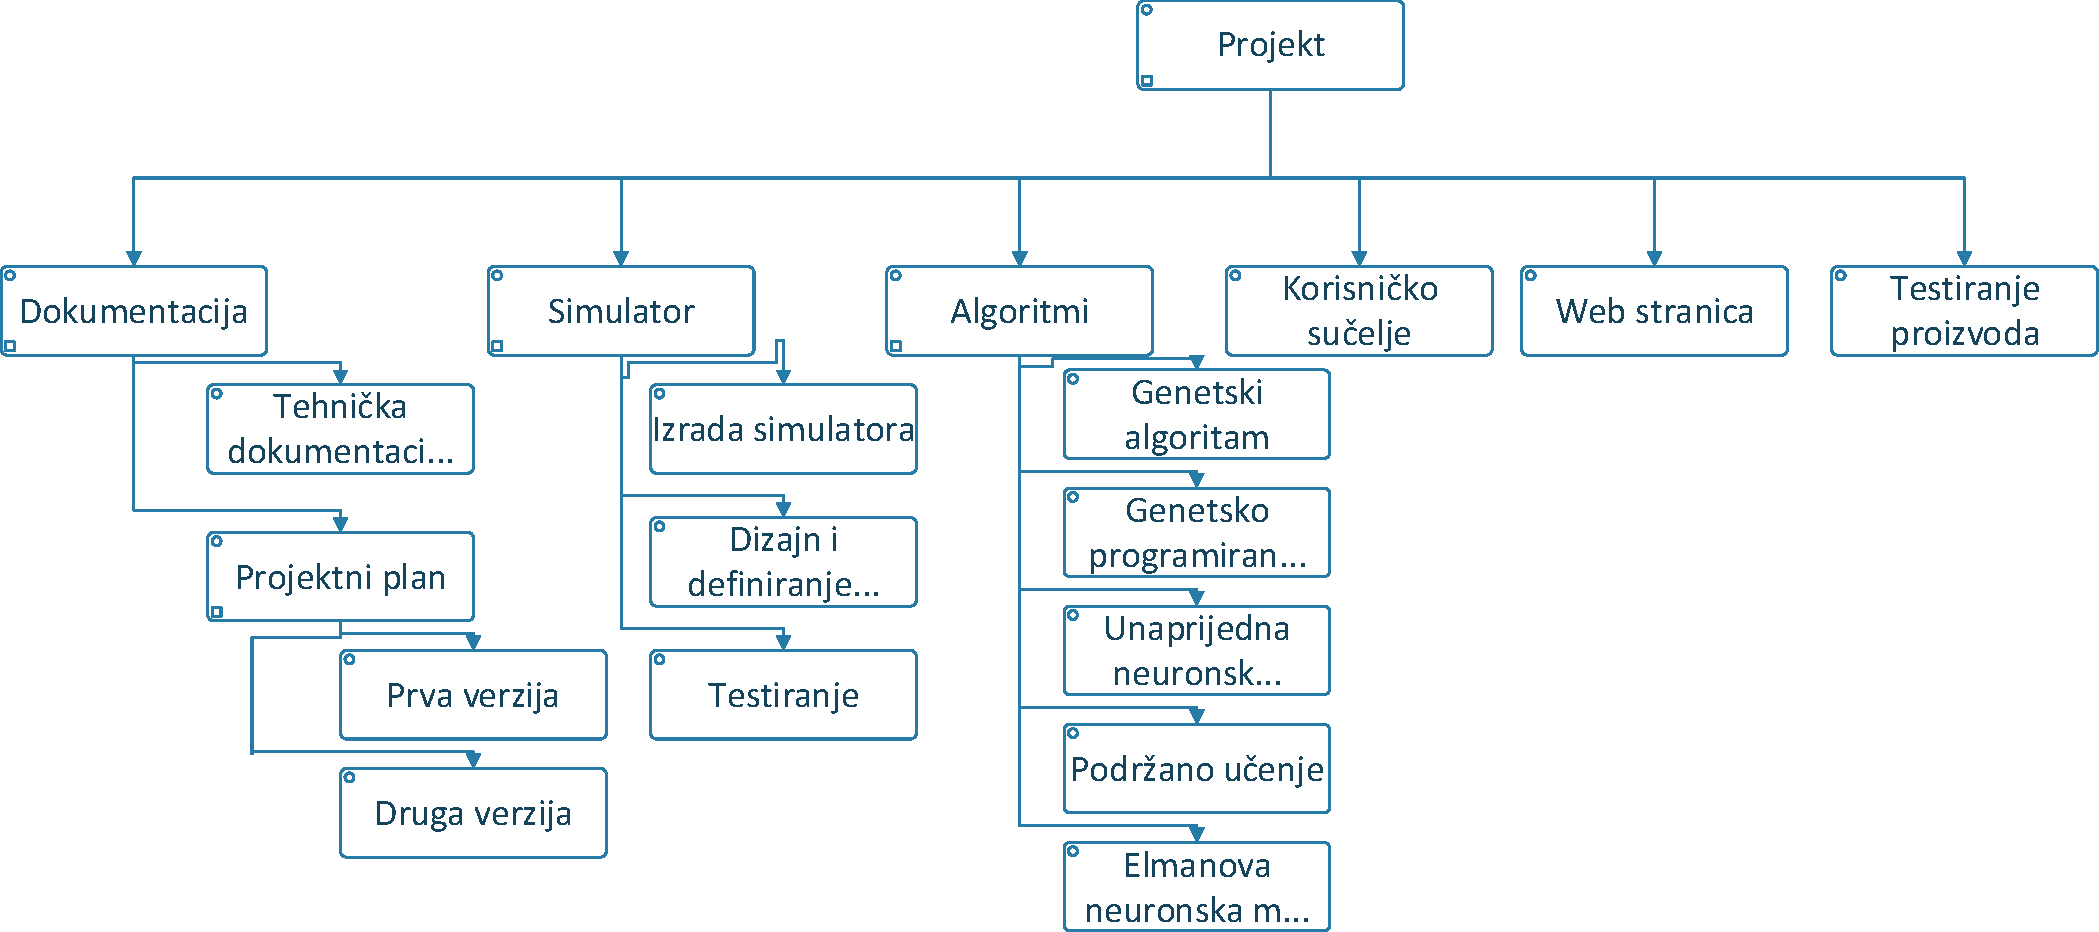
\includegraphics[scale=0.55]{WBS.pdf}
\caption{Struktura raspodijeljenog posla}
\end{figure}

 
\section{Kontrolne točke}
\begin{table}[H]
\centering
 \begin{tabular}{||l c c c||} 
 \hline
 Kontrolne točke & Planirani datum & Realizirani datum & Status projekta \\ [0.5ex] 
 \hline\hline
 Izrada simulatora & 20.10.2016. & 20.10.2016. & Simulator izrađen \\ 
 Prva verzija projektnog plana & 07.11.2016. &  07.11.2016. &  Projektni plan usvojen\\
 Izrada algoritama & 02.01.2016. &  &  \\
 \begin{tabular}{@{}l@{}}Izrada korisničkog sučelja \\ Druga verzija projektnog plana \\ Tehnička dokumentacija  \end{tabular} & 09.01.2016. &   &\\
 Završetak izrade web-stranice & 16.01.2016. &  &  \\
 \hline
 \end{tabular}
 \caption{Kontrolne točke projekta}
\end{table}


\section{Gantogram}
\begin{figure}[H]
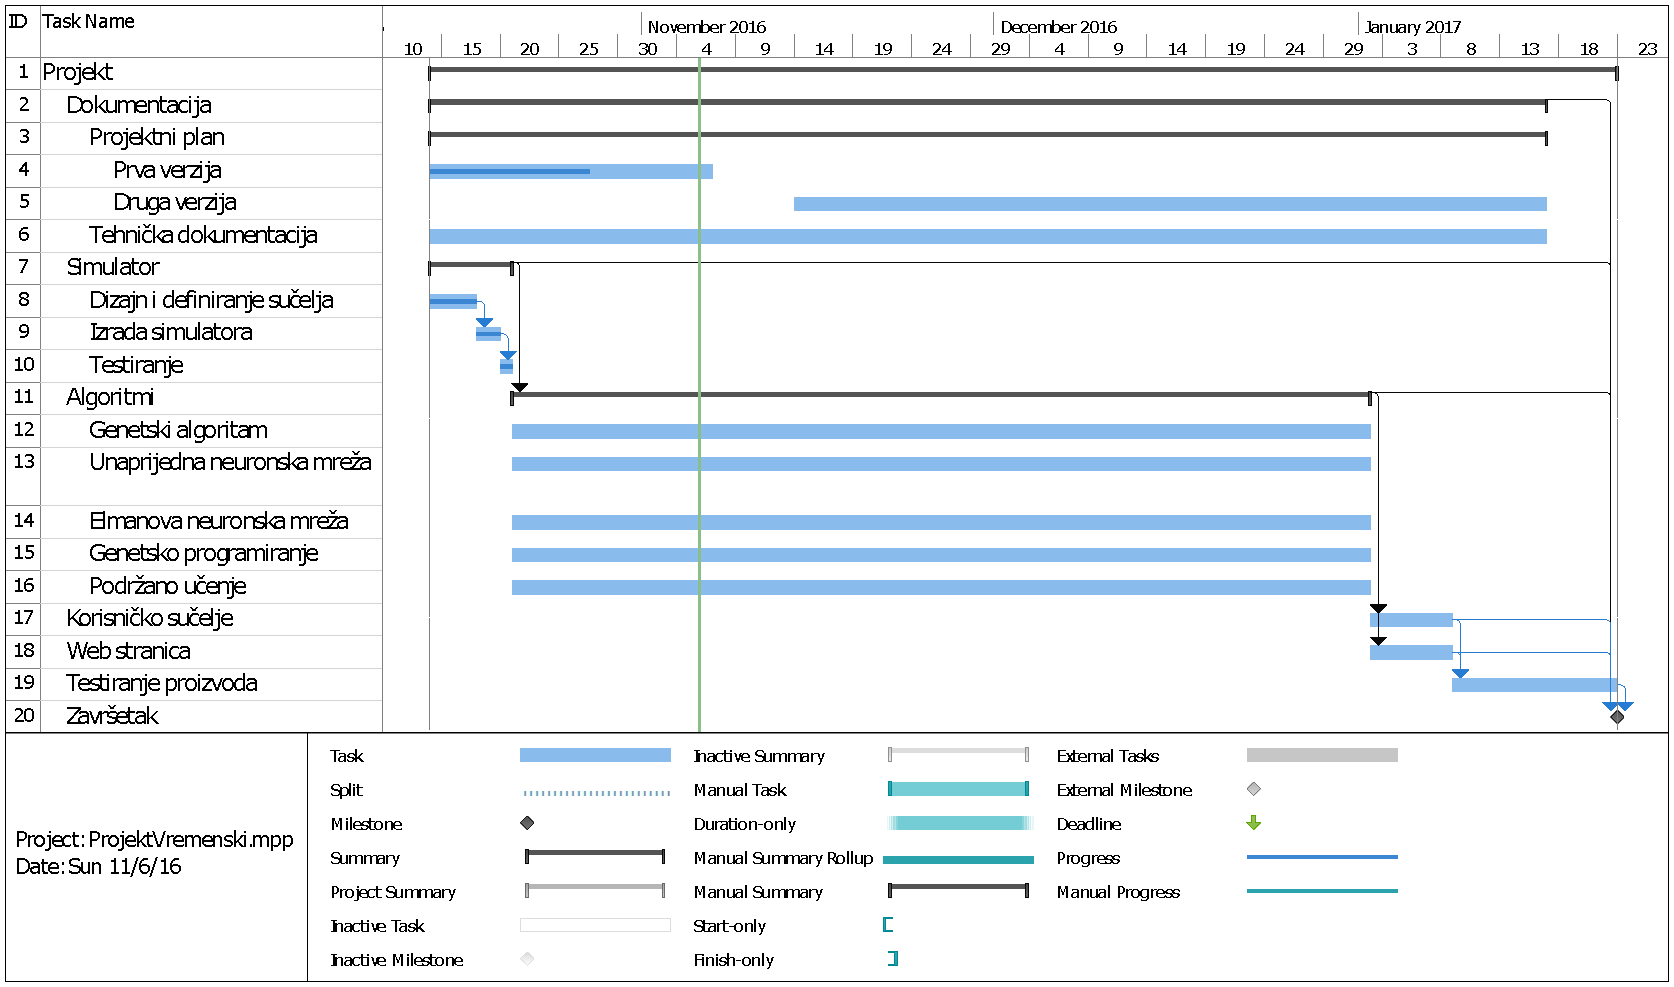
\includegraphics[scale=0.57]{ProjektVremenski.pdf}
\caption{Gantogram}
\end{figure}

\section{Zapisnici sastanaka}
\begin{table}[H]
\centering
 \begin{tabular}{||c c c||} 
 \hline
 Datum & Prisutni & Zaključci\\ [0.5ex] 
 \hline\hline
 14.10.2016. & svi članovi tima & Inicijalni sastanak, raspodijela poslova\\
 17.10.2016. & svi članovi tima & Dogovor oko izrade simulatora\\
 07.11.2016. & svi članovi tima & Prihvaćena prva verzija projektnog plana\\
 \hline
 \end{tabular}
 \caption{Zapisi sastanaka}
\end{table}

\end{document}